\section{On image correction}
\label{imaging:correction}

Fluorescence microscopy images contain non-biological data,
distortions, and artifacts that may confound analytical results if
not addressed.
In the terms of the image model from the previous section
(\ref{eq:imaging:simpleFullModel}), the
subject of study in fluorescence imaging is contained within a subset of the
foreground layers. All non-foreground components should thus
be removed in order to obtain meaningful quantitative results.
Ideally, the foreground layers that are not of interest (especially
artifacts) should also be removed, though this is a much more difficult
problem that I do not address in this dissertation.
In essence, from the original image $I=D+S(F+B)\epsilon$, we need to
obtain $F$: obtaining $F$ is the goal of image correction.


It is important to be aware that image correction is not a solved
problem. There are many ways in which it can be done, several of which I review
in \ar{imaging:correction:review}, but the most commonly-used methods produce
incomplete correction and/or are prone
to generating artifacts. Further, methods sections of papers that
rely on imaging often do not explain their correction methodology
at all, making it difficult to evaluate some published results.
I therefore make the importance of image correction a focus
of this chapter, and describe an image correction
approach that I developed for accurate determination of $F$
in the difficult context of high-throughput microscopy
\ar{imaging:correction:myMethod} \cite{Coster2014}.


Before going into the details of image correction, I should
first address whether this step is even necessary.
After all, any processing step
could introduce artifacts and thus potentially do more harm than good.
Normal cell-to-cell variability is already relatively high,
with standard deviations of 
$\sim$15-30\% for protein concentrations \cite{Sigal2006a}. One might then
wonder whether error introduced by non-foreground image components
would make much of a difference. Here I show that it can
indeed make a difference. Unsurprisingly,
the size of the difference (and thus the importance) is highly
dependent on the properties of each particular image dataset,
the measurement methods used, and the experimental goals.


\subsection{Non-foreground components distort single-cell phenotypes}
\label{imaging:distortion}


A particular cellular phenotype can be represented
as a set of measurements.
For example, a cell phenotype might be composed of
its measured size, shape, texture,
and average fluorescence intensities in multiple
color channels. Each measurement is
generally referred to as a ``feature.'' The diversity
of features that can be measured
for a  single cell is only limited by the imagination
of the investigator. It would therefore
be impossible to develop a single
comprehensive argument for the importance
of image correction that covers all possible
ways of measuring cellular phenotypes.
Instead, I make a case study of several
commonly-used and biologically-interpretable
single-cell features: the average, total,
and ratios of fluorescence intensity.


    \begin{table}[!bt]
    \caption[Table of symbols for average, total, and ratiometric features.]
    {Symbols used in the mathematical derivations of the consequences of $S$
    and $B$ on single-cell feature distributions.}
    \label{table:imaging:symbols}
    \centering
    \begin{tabular}{cl}
    \hline
    Symbol & Meaning \\ \hline
    $\E[X]$   & Expected value (i.e. the mean) of the random variable $X$ \\
    $F_c$	 & Average foreground intensity within cell $c$ \\
    $S_c$	 & Average shading value within cell $c$ \\
    $B$	     & Background intensity per pixel, a constant\\
    $\alpha_c$ & Area of cell $c$ \\
    $A$	     & Average intensity feature \\
    $T$	     & Total intensity feature \\
    $R$	     & Ratio of intensities feature \\
    $Z_c$    & The value of feature $Z$ for a single cell, $c$.\\
    $\sigma_Z$ & The standard deviation of feature $Z$ across all cells. \\
    $\mu_Z$    & The mean of feature $Z$ across all cells. \\
    $cv_Z$     & The coefficient of variation of feature $Z$ across all cells  ($\sigma_Z/\mu_Z$). \\
    \hline
    \end{tabular}
    \end{table}


How to quantify the effects of image correction on data is not obvious,
since that data can be used in many ways depending on experimental goals.
There are, however, aspects of
single-cell distributions that are meaningful across a broad array of
experiments, and so I use these as metrics when measuring the consequences
of image correction. These are the mean ($\mu$), standard deviation ($\sigma$),
and coefficient of variation ($cv=\sigma/\mu$) of a feature across a population of cells.


The standard deviation and $cv$ are measures of distribution widths, which
are used to determine the statistical separability of distributions.
Inaccurate measurements of the true variability may
consequently reduce statistical power.
The mean of a feature distribution, on the other hand,
is typically used to determine how large of an
effect an experimental perturbation has had. Inaccurate measurements of the true mean
may cause strong results to appear weak, or vice versa, leading to false
negatives or false positives. These distribution metrics are
therefore useful as readouts for the utility of image correction.


The mathematics in the following discussion were
worked out in conjunction with my co-authors on the relevant
publication \cite{Coster2014}: Satwik Rajaram, Chonlarat Wichaidit,
Steven Altschuler, and Lani Wu. The text
and figures draw heavily from the same publication. Those readers
who do not need convincing that image correction is important may skip
to page~\pageref{imaging:correction:review} without a loss in coherence
of this chapter.


  \begin{figure}[!bt]
  \centering
  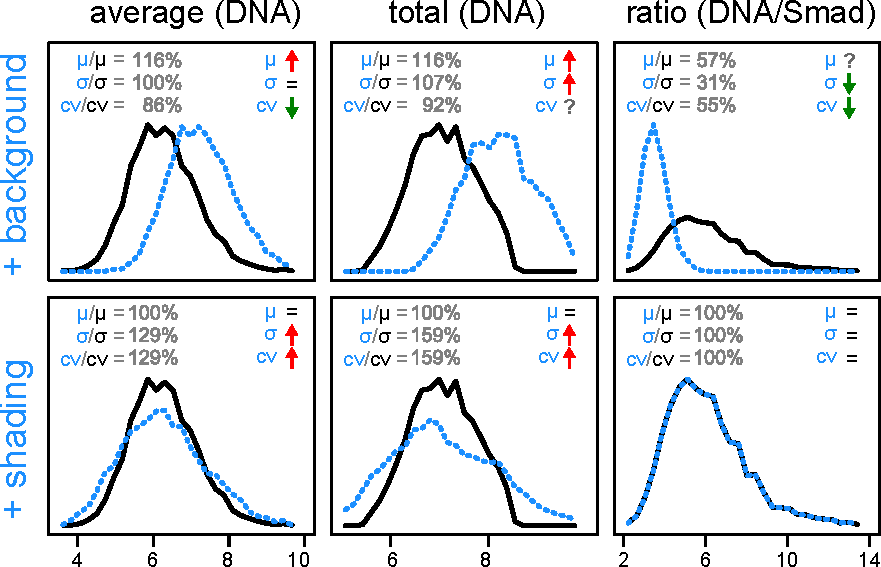
\includegraphics[width=4.5in]{FIGS/imaging/SBeffects.pdf}
  {\singlespacing 
  \caption[ Case study of the effects of $S$ and $B$ on single-cell features.]
            { Image background and shading cause feature-dependent changes
            in estimates of phenotypic variability.
            Human colonic epithelial cells ($n>3700$), stained for DNA
            (using Hoechst) and Smad (using a Smad2/3 antibody), imaged
            at 10X.
            The distributions of
            nuclear feature values were then compared
            before (black histograms) and after (dotted blue histograms)
            artificial background (top row, with
            background $\sim$16\% of Hoechst or $\sim$50\% of Smad foreground)
            or shading (bottom row, linear
            gradient with maximum 1.5 fold intensity difference) were added
            to each image. $\mu$, mean; $\sigma$, standard deviation;
            $cv=\sigma/\mu$. Inset, top left,
            relative size of change to the shown distributions. Inset, top right,
            arrows indicate the direction of
            change in the general case (question marks indicate uncertainty due to
            dependency on other variables). $x$-axes in arbitrary fluorescence units.
            A version of this figure is published as Fig. 1a in \cite{Coster2014}.}
  \label{fig:imaging:SBeffects}}
  \end{figure}





\subsubsection{Mathematical definitions of commonly used single-cell features}


Commonly used single-cell measurements include pixel intensity averages,
totals, and ratios within some cellular compartment $c$ (such as the
nucleus, cytosol, or whole cell).
By defining these features mathematically we
can determine their general behaviors as a consequence of the presence of image background
or shading. Refer to \ar{table:imaging:symbols} for the list of mathematical
symbols, to \ar{table:imaging:properties} for a summary of the statistical
properties used in the mathematical derivations, and
\ar{fig:imaging:SBeffects} for a case study of these behaviors.


For each cellular object, I define $F_c$ and $B_c$ as the average foreground
and background intensities within $c$, while $S_c$ is the
average shading. $B_c$ is a constant for all cells,
as the background is assumed to be the same for all
pixels in the absence of noise, and so I drop the subscript from this term.
I refer to the area of each cell, measured in pixels, as $\alpha_c$.
Finally, for the derivations I assume that the detector value has
been subtracted from all pixels
and that the image contains no measurement noise  ($D=0$
and $\epsilon=1$).


For each cell I can then define the three simple intensity features: total intensity $T$,
average intensity $A$, and the ratio of intensities $R$ between two independent foreground
signals $F_{c1}$ and $F_{c2}$ (e.g. the ratio of nuclear Hoechst and Smad intensities, as in
\ar{fig:imaging:SBeffects}). Because the ratio takes two signals into account, each may
come from a distinct fluorophore and optical setup and so have 
distinct shading and background values. Additionally, those features could be
defined within distinct cellular compartments, such that the compartment
sizes may also differ.
The three features are thus defined for single cells by 
Equations~\ref{eq:correction:average}\nobreakdash-\ref{eq:correction:ratio}.
	%
	\begin{align}
	A_c & = S_c (F_c+B) \label{eq:correction:average}\\
	T_c & = \alpha_c A_c = \alpha_c S_c (F_c+B) \label{eq:correction:total}\\
	R_c & = \frac{ \alpha_{c1} S_{c1}(F_{c1}+B_1) }{ \alpha_{c2} S_{c2}(F_{c2}+B_2) }  \label{eq:correction:ratio}
	\end{align}
	

For simplicity of the following analysis, I take the special case where
$F_c$, $S_c$, $\alpha_c$, and $B$ are all
statistically independent (i.e. cells do not
spatially arrange themselves within an image
by phenotype, and foreground intensity is
independent of cell size). Further, I
assume that cells are small relative to the
spatial rate of change of $S$ across an image.
These assumptions 
allow me to use the properties in
\ar{table:imaging:properties}. Note that these assumptions
will be valid for some experimental cases, but
certainly not all. For the case study
shown in \ar{fig:imaging:SBeffects} they are appropriate:
I verified that nuclear size and staining intensity
were uncorrelated with each other and with position, and that the two
foreground signals (Hoechst and Smad2/3) are independent (data not shown).


Finally, I noted earlier that units of fluorescence are typically arbitrary
and that $S$ causes a multiplicative change in relative intensity across
an image. This means
that we are free to choose how to define the expected value of $S$: a
value other than 1 would cause a scaling of the foreground and
background values, but this scaling would retain the relative relationship between
all measured intensities and so would be of no consequence.
For convenience, then, I define shading so that
its expectation value across all images and pixels is $\E[S]=1$
so that, for a large number of cells, $\E[S_c]\approx 1$. This definition simplifies
the mathematical derivations below, as the $\E[S_c]$ term can be dropped
from several formulae.


    \begin{table}[!bt]
    \centering
    \caption[Table of useful statistical properties.]{
    Statistical properties used in the derivations of the effects
    of shading $S$ and background on the distributions of single-cell
    average $A$, total $T$, and ratio $R$ intensity features. $X$ and $Y$ are independent
    random variables, and $k$ is a constant.}
    \label{table:imaging:properties}
    \begin{tabular}{ccl}
    \hline
    Index & Property \\ \hline
    1 & $\E[S_c] \equiv 1$  \\
    2 & $\mu_{X+k} \equiv \E[X+k] = \E[X]+k$ \\
    3 & $\mu_{XY} = \E[X]\E[Y]$ \\
    4 & $\sigma^2_X \equiv \Var[X] = 
        \E[X^2]-\E[X]^2 \implies \E[X^2]\geq \E[X]^2$\\
    5 & $\sigma^2_{[X+k]} = \sigma^2_X$ \\
    6 & $\sigma^2_{XY} = \E[X^2]\E[Y^2]-\E[X]^2 \E[Y]^2$ \\
    \hline
    \end{tabular}
    \end{table}



\subsubsection{Effects of background $B$ on the average intensity feature $A$}


For this case, we ignore the effects of $S$ and focus on $B$. 
We therefore set $B>0$ and $S_c=1$, so that the average feature 
from \ar{eq:correction:average} simplifies to $A_c=F_c+B$.
This results in the distribution properties for this feature in 
Equations~\ref{eq:correction:bamu}\nobreakdash-\ref{eq:correction:bacv}.
	%
    \begin{align}
    \mu_A    & \equiv \E[A_c] = \E[F_c+B] = \E[F_c] + B  \label{eq:correction:bamu}\\
    \sigma_A & \equiv \sqrt{\Var[A_c]} = \sqrt{\sigma^2_{F_c+B}} = \sigma_{F_c} \label{eq:correction:basd}\\
    cv_A     & \equiv \frac{\sigma_A}{\mu_A} = \frac{\sigma_{F_C}}{\E[F_c]+B} \label{eq:correction:bacv}
    \end{align}


It is clear that $B$ will always cause
an increase in the mean of average intensities, $\mu_A$ \arp{eq:correction:bamu}.
The standard deviation, $\sigma_A$, is
unaffected by background (\ar{eq:correction:bamu}, using Property 5 from \ar{table:imaging:properties}).
As a consequence of the
constant $\sigma_A$ and increased $\mu_A$, the coefficient of variation
will decrease with increasing background. In summary, background will cause
an overestimation of $\mu_A$, an underestimation of $cv_A$, and will not affect
$\sigma_A$ (ee the case study in \ar{fig:imaging:SBeffects}, top left panel).


\subsubsection{Effects of background $B$ on the total intensity feature $T$}


The situation is the same as the previous case,
except with the inclusion of cell size.
The total intensity feature \ar{eq:correction:total}
therefore simplifies to $T_c=\alpha_c (F_c+B)$,
resulting in the distribution properties shown in 
Equations~\ref{eq:correction:btmu}\nobreakdash-\ref{eq:correction:btcv}.
	%
    \begin{align}
    \mu_T    & \equiv \E[T_c] = \E[\alpha_c(F_c+B)]=\E[\alpha_c](\E[F_c]+B) =
        \E[\alpha_c]\E[F_c]+\E[\alpha_c]B
        \label{eq:correction:btmu}\\
    \sigma_T & \equiv \sqrt{\Var[T_c]} = \sqrt{\sigma^2_{\alpha_c(F_c+B)}} =
        \sqrt{\sigma^2_{\alpha_c F_c} + 2\sigma^2_{\alpha_c}\E[F_c]B
        + \sigma^2_{\alpha_c}B^2}
        \label{eq:correction:btsd}\\
    cv_T     & \equiv \frac{\sigma_T}{\mu_T} =
        \frac{ \sqrt{\sigma^2_{\alpha_c F_c}+2\sigma^2\E[F_c]B+ \sigma^2_{\alpha_c}B^2 } }
        { \E[\alpha_c]\E[F_c] + \E[\alpha_c]B }
        \label{eq:correction:btcv}
    \end{align}

    
Though somewhat less obvious than for the average feature,
it should be clear that increasing $B$ will cause
an increase in the mean of total intensities, $\mu_T$
(\ar{eq:correction:btmu}, using Property
3 from \ar{table:imaging:properties}). Importantly,
each cell will be affected differently by background, depending on its size.
Unlike the average feature, the standard deviation $\sigma_T$
increases with background (\ar{eq:correction:btsd},
using Properties 3 \& 6 from \ar{table:imaging:properties}).


Because both $\sigma_T$ and increased $\mu_T$ increase with
increasing $B$, it is not immediately obvious what the effect should be on the
coefficient of variation, $cv_T$ (as the numerator and
denominator in \ar{eq:correction:btcv} both are proportional to $B$).
However, if we take the derivative of the $cv$ with respect to a changing
background, we get \ar{eq:correction:btcvdb}. Because this derivative
is always $\leq 0$, the $cv_T$ will decrease with increasing
background. In summary, background will cause
cell size-dependent overestimation of $\mu_T$ and $\sigma_T$,
and underestimation of $cv_T$ (see the case study in
\ar{fig:imaging:SBeffects}, top middle panel).
	%
    \begin{equation} \label{eq:correction:btcvdb}
    \frac{d}{dB}(cv_T^2)= -2 \frac{ \sigma^2_{F_c}\E[\alpha_c^2] }
        { \E[\alpha_c]^2(\E[F_c]+B)^3 } \leq 0
    \end{equation}


\subsubsection{Effects of shading $S$ on the average intensity feature $A$}


We now move on to the effects of shading on the average and total features,
and therefore set $B=0$. Note that increasing the magnitude of $\E[S_c]$
will have no effect on any of these features, as it is the same as a change in
units. Because shading is a variation in intensity across an image,
we can therefore modulate its strength by
changing the variance of this image component.
The larger the variance, the more shading. For this case, then,
we set $\Var[S_c]>0$.
The average intensity feature from \ar{eq:correction:average} therefore
simplifies to $A_c=S_c F_c$.
This results in the distribution properties shown in 
Equations~\ref{eq:correction:samu}\nobreakdash-\ref{eq:correction:sacv}.
	%
    \begin{align}
    \mu_A    & \equiv \E[A_c] = \E[S_c F_c] = \E[S_c]\E[F_c]=\E[F_c]
        \label{eq:correction:samu}\\
    \sigma_A & = \sqrt{\sigma^2_{S_c F_c}} =  \sqrt{ \E[S_c^2]\E[F_c^2]-\E[S_c]^2\E[F_c]^2 }
        = \sqrt{ \E[S_c^2]\E[F_c^2]-\E[F_c]^2 }
        \label{eq:correction:sasd}\\
    cv_A     & \equiv \frac{\sigma_A}{\mu_A} = \frac{ \sqrt{\E[S_c^2]\E[F_c^2]-\E[F_c]^2} }
        { \E[F_c] }
        \label{eq:correction:sacv}
    \end{align}

From \ar{eq:correction:samu} it is obvious that $S$ has no effect on
the mean of average intensities, $\mu_A$, as it falls out of the formula entirely
(using Properties 1 \& 3 from \ar{table:imaging:properties}).
The standard deviation, $\sigma_A$, however will increase
with background (\ar{eq:correction:sasd},
using Properties 1, 4, \& 6 from \ar{table:imaging:properties}).
As a consequence of the
increasing $\sigma_A$ and constant $\mu_A$, the coefficient of variation
increases with increasing background. In summary, shading will cause
overestimation of variation for $A$
(see the case study in \ar{fig:imaging:SBeffects}, bottom left panel).
Shading does not affect $\mu_A$, but this
is not surprising since I defined shading to have a mean of 1 specifically
so that it would not affect the mean.
    
    

\subsubsection{Effects of shading $S$ on the total intensity feature $T$}


The situation is the same as the previous case, except with the inclusion of cell size.
The total intensity feature \ar{eq:correction:total}
therefore simplifies to $T_c=\alpha_c S_c F_c$.
This results in the total intensity distribution properties shown in 
Equations~\ref{eq:correction:stmu}\nobreakdash-\ref{eq:correction:stcv}.
	%
    \begin{align}
    \mu_T    & \equiv \E[T_c] = \E[\alpha_c S_c F_c] = \E[S_c]\E[\alpha_c F_c]=
        \E[\alpha_c]\E[F_c]
        \label{eq:correction:stmu}\\
    \sigma_T & = \sqrt{\sigma^2_{S_c F_c}} =  \sqrt{ \E[S_c^2]\E[\alpha_c^2 F_c^2]-
        \E[S_c]^2\E[\alpha_c F_c]^2 }
        = \sqrt{ \E[S_c^2]\E[\alpha_c^2 F_c^2]-\E[\alpha_c F_c]^2 }
        \label{eq:correction:stsd}\\
    cv_T     & \equiv \frac{\sigma_A}{\mu_A} = \frac{ \sqrt{\E[S_c^2]\E[\alpha_c^2 F_c^2]-
        \E[\alpha_c F_c]^2} }
        { \E[\alpha_c F_c] }
        \label{eq:correction:stcv}
    \end{align}


The derivation is nearly the same as that for the
previous case for the average feature.
As before, from \ar{eq:correction:stmu} we see that $S$ has no effect on
the mean of total intensities, $\mu_T$. Also as before,
the standard deviation, $\sigma_T$, will increase
with shading, as will $cv_T$
(see the case study in \ar{fig:imaging:SBeffects}, bottom middle panel).
Thus, increasing the shading always artificially
increases the variation of the average and total intensity features.



\subsubsection{Effects of $B$ and $S$ on $R$}


I now turn to the ratiometric feature \arp{eq:correction:ratio}, 
which turns out to be
the least generalizable even within the narrow constraints defined
at the start of this section. And so to simplify, I further constrain
the discussion to the ratio of average intensities. This allows us
to set $\alpha=1$ for both signals (note that these terms also
cancel when taking the ratio within a single compartment). Thus, we have
\ar{eq:correction:ratioMeans}.
	%
	\begin{equation} \label{eq:correction:ratioMeans}
	R_c = \frac{ S_{c1}(F_{c1}+B_1) }
	{S_{c2}(F_{c2}+B_2) } 
	\end{equation}


There are a few distinct cases we can examine to get an idea of
how this ratio behaves. In the first case, we can have the signals
originating from the same channel (for example, the ratio of
nuclear to cytosolic Smad2/3). Here, $B_1=B_2$ and, under my
earlier assumption that cells are small relative to the rate
of change of $S$, $S_{c1}=S_{c2}$. The ratio thus becomes
$R_c=\frac{F_{c1}+B}{F_{c2}+B}$ and is unaffected by shading.
The effects of $B$ are less obvious because it
is in both the numerator and denominator. In the limiting case,
however, $\lim_{B\rightarrow \infty} R_c=1$. Since all values
are forced to 1 with large $B$, the variation across the population
will be forced to 0. In less extreme
cases, however, background can either cause an increase
or decrease in
the apparent variation, depending on its size relative to
both foreground terms. Because of this, the error in the
measured ratio can vary from cell to cell within the same
population. For example, if two cells have the same ratio
but different absolute foreground values, $B$ will cause their
ratios to diverge (e.g. $\frac{1+B}{2+B}\neq\frac{10+B}{20+B}$).
This effect causes the scrambling seen in \ar{fig:imaging:backgroundRatio}.


  \begin{figure}[!bt]
  \centering
  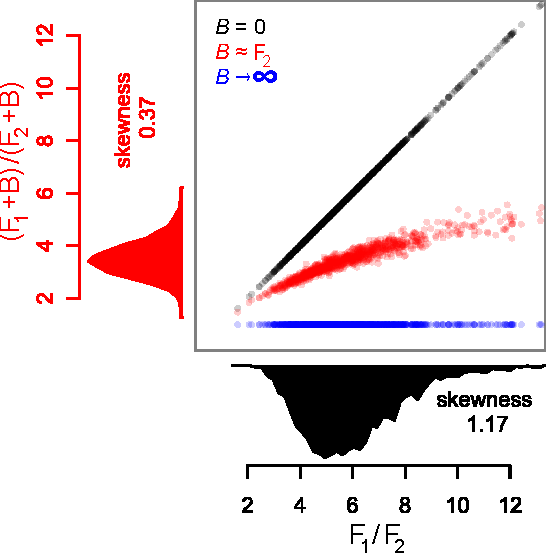
\includegraphics[width=3in]{FIGS/imaging/backgroundRatio.pdf}
  {\singlespacing 
  \caption[ Idiosyncratic effects of background on ratiometric features.]
            { Ratiometric features are idiosyncratically affected by background.
            The same initial data as in the right panels of \ar{fig:imaging:SBeffects},
			but where each single-nucleus ratio
            after addition of background is plotted against its true value (1000/3700 cells shown).
            To each average was added 0 (black), 1000 (red),
            or $10^{10}$ (blue) background units before taking the ratio. The first
            two artificial cases are the same as those in \ar{fig:imaging:SBeffects}.
			The impact on the apparent ratio
            is dependent on the relative sizes of the foregrounds and the background,
            such that the data becomes scrambled in the red curve.
            Note that
			the distribution shape is also affected, such that adding background
			decreased the skewness. $F_1$, average
            single-nuclear Hoechst; $F_2$, average nuclear Smad2/3.}
  \label{fig:imaging:backgroundRatio}}
  \end{figure}


In the second case, we could allow $F_{c1}$ and $F_{c2}$ to come
from distinct channels, which would also allow them to have
different shading
and background. As a consequence, the effects on the
distribution properties are extremely difficult to predict
due to the presence of many independent variables
(as indicated in the case study in \ar{fig:imaging:SBeffects}, right panels).
I therefore leave the discussion here, with
the conclusion that the mean and variation of the ratio feature can both
increase or decrease with different ranges of component values.
This unpredictability has important
ramifications for applications such as
fluorescence resonance energy transfer (FRET) where interpretation
relies on accurate cross-channel ratios \cite{Hodgson2010}.


\subsubsection{On the importance of image correction}

Unfortunately, the mathematical discourse above leaves us
with the dissatisfying result that the importance of image correction
is highly dataset dependent. In \ar{fig:imaging:SBeffects} I show
the size of the distortion for an example dataset with
experimentally-reasonable amounts of background and shading, which
shows effects that are measurable and sometimes relatively large. However,
different analytical requirements can tolerate quite different
amounts of feature distribution distortion before
data interpretation is affected.
The best I can do then, besides the easy blanket statement
``always correct your images!'' is to provide a few rules of thumb for
deciding on the importance of image correction.


First, I
completely ignored the detector contribution ($D$) in the above
discussion because
the matrix $D$ is unchanging and is therefore trivial to subtract from
images. Removal of $D$ should be a part of all image
analysis pipelines. This step is rarely explicitly performed
in the literature but can have a large impact
on measurements of weakly-fluorescent samples. In particular,
shading will be underestimated without subtraction of the detector
fluorescence contribution.


Second, shading tends to increase feature distribution widths
and so should be corrected whenever measurement of true biological
variability is important. Additionally, if the foreground to background ratio
is low, then shading may cause foreground values in one part of an image to fall below
background values in another part. This can have
important consequences to image segmentation \arp{imaging:segmentation}
\cite{Herbert2012}. However, in the case that biological
variability is high relative to the variation in shading
it would not be necessary to correct for $S$.
This is because the observed average and total distributions are
the convolution
of the shading and foreground distributions. If two normal distributions
with variances $\sigma^2_1$ and $\sigma^2_2$ are convolved, they yield a new
distribution with $\sigma^2_3=\sigma^2_1+\sigma^2_2$. Because shading
is a relative term, we have to scale it to the size of $F_c$ to make
use of this property: $\sigma^2_{\text{observed}}=(F_c\sigma_{S_c})^2+\sigma_{F_c}^2$.
Thus, if $F_c\sigma_{S_c}^2<<\sigma_{F_c}^2$ the observed
distribution will be close to the true distribution. While this
is a useful rule of thumb, I note that I have never observed normally-distributed
shading values (see examples in \ar{fig:imaging:properties}b).


Third, background can dramatically shift feature distribution
means. Background should therefore be corrected either when accurate means
or accurate ratios between two means are needed. When background
is low compared to even the lowest foreground values, however, it will have
little impact on the feature distributions discussed above.


Finally, when using cross-channel ratios extra care should be
taken to ensure that both background and shading are corrected.
These ratios should always be interpreted with an eye towards
the possible
effects of imaging artifacts, as artifacts can distort rations
in unpredictable ways.


\subsection{Review of image correction methods}
\label{imaging:correction:review}


Now that I have given some motivation for the importance of image correction, 
I turn to the available methods for this
process. Here, I briefly review the correction methods that
are commonly employed in the literature. In general, when deciding
on a method the investigator should test its theoretical performance
given the image model described in this chapter, $I=D+S(F+B)$.
By taking this approach, deficiencies or important assumptions of
the methods should become clear.


There are many published methods for fluorescence image correction,
perhaps as many methods as there are labs, due to the idiosyncrasies
of imaging data and the lack of standardized approaches.
I group the most common methods into two broad, non-exhaustive
categories, which I refer to as ``reference-image'' and ``per-image''
correction.
Reference-image methods obtain correction parameters from one image
and then use those parameters to correct another image. Per-image methods
find such parameters in the very image that is to be corrected.


Reference-image methods are straightforward and so are commonly used and 
recommended throughout the literature
\cite{VandenDoel1998,Model2001,Zwier2004,Wolf2007,Waters2009}.
These methods make a key assumption: that the reference image 
has approximately the same shading and background
as do the images to be corrected. A good example of this approach
uses two reference images to flatten shading, subtract background,
and normalize the fluorescence
intensity to a standard \cite{Model2001}.
One reference image, $I_\text{uniform}$ contains a
dissolved fluorophore; because this image would be flat without shading, it can
be used to determine how much shading is present in the real images. The other
reference, $I_\text{background}$ is the same as the sample images but contains no
sample. This image can thus be used to estimate background.
Equations~\ref{correction:example1}\nobreakdash-\ref{correction:example2} demonstrate this method.
	%
	\begin{align}
	I_\text{sample}     &= D+S(F_\text{sample}+B) \label{correction:example1}\\
	I_\text{background} &= D+SB \label{correction:ib} \\
	I_\text{uniform}    &= D+S(B_\text{uniform}+B) \\
	I_\text{corrected}  &= \frac{ I_\text{sample}-I_\text{background} }{ I_\text{uniform}-I_\text{background} }
		= \frac{ [D+S(F_\text{sample}+B)]-[D+SB]}{ [D+S(B_\text{uniform}+B)]-[D+SB] }
		= \frac{F_\text{sample}}{B_\text{uniform}} \label{correction:example2}
	\end{align}
	


While reference-image methods are straightforward and often easy to perform,
some of those recommended in the literature are only partially corrective. This is especially
true with respect to the detector value $D$, which
I have not seen explicitly accounted for in these methods.
To find out if a given method performed complete correction, investigators can plug the
image model into the method and check that, algebraically, the output is either
$F$ or some normalized form of it (as in \ar{correction:example2}).
However, note that partial correction may be
sufficient in some cases, particularly when background intensity is low compared
to foreground intensity and when within-image shading variation
is low compared to foreground variation.


Per-image methods, on the other hand, have the challenging task of measuring
all image components ($D$, $S$, $F$, and $B$)
within the image that is to be corrected. These methods typically
work by trying to fit a model to the combination of non-foreground
layers, $D+SB$. Therefore the primary difficulty
is that images typically contain varying fractions of foreground pixels
(e.g. due to variation in cell density),
so that determination of which pixels consist of background
is non-trivial. Further, even if identification of background pixels
is straightforward within an image, the size of the background signal
``underneath'' a foreground object is necessarily unknown and must
be predicted. The method for this prediction is what separates the different
per-image correction algorithms. 


Some per-image methods fit a polynomial \cite{L2000}
or spline surface \cite{Lindblad162266,Lindblad2004,Yin2013} to predicted
non-foreground pixels, therefore assuming a 
particular structure to the shading patterns.
These methods may also assume properties of 
the foreground objects (e.g. fluorescing cells),
such as a maximum size in the case of the rolling ball algorithm employed by
ImageJ\cite{Schneider2012} and Fiji \cite{Schindelin2012},
and may perform non-linear transformations of the underlying
images. Additionally, the accuracy of these
approaches necessarily decreases with
increasing cell density as there are fewer
background pixels from which to estimate
$I_\text{background}$. High confluency or cell clumping can thus cause
per-image methods to introduce artifacts.


When they work properly, per-image based methods generate
$I_\text{background}$ \arp{correction:ib} 
from each sample image, $I_\text{sample}$ \arp{correction:example1}.
From this point, then, the reference-based and per-image based
correction methods are the same; the only difference is in how
$I_\text{background}$ is obtained.
The question that then remains in both cases is which
mathematical operation to perform in order to correct the sample images. 
In the literature,
subtraction ($I_\text{sample}-I_\text{background}$) is frequently
used. However, subtraction does not remove
shading, as the algebraic result is $SF$ instead of $F$. The standard
rolling ball algorithm employed by ImageJ and
FIJI uses this subtractive approach.


The better approach is to use division to remove shading. This can be
done in combination with subtraction to remove both background and shading,
as in the example above \arp{correction:example2}. However, many studies
use simple division ($I_\text{sample}/I_\text{background}$), which results
in $\frac{D+S(B+F)}{D+SB}=1+\frac{SF}{D+SB}$. This result is a
background-normalized foreground with incompletely-corrected shading.
The correction can be completed by prior subtraction of $D$ from both images,
followed by subtraction of 1, which would yield the normalized image $F/B$.


I use a different approach from those listed above, 
which is to independently estimate all
non-foreground parameters so that I can perform the image algebra
that expicitly returns $F$. I discuss this method next.


\subsection{An improved correction method for high-throughput imaging}
\label{imaging:correction:myMethod}


Having determined the importance of image correction, and observed
the diversity and frequent inaccuracy of the available correction methods,
I sought to develop a simple and robust method for my own imaging applications.
All of the work in this dissertation took advantage of the throughput of
microtiter plates (e.g. 96- and 384-well plates), and so in particular I needed
to be able to accurately correct large numbers of images with
minimal computational overhead.
Further, I needed the correction to be robust to cell density,
so that I could correctly measure single-cell biological variability
under a wide variety of experimental conditions.


The approach that I developed (published in \cite{Coster2014}),
is a reference-based
method that relies on a key observation: shading patterns
are highly predictable
in microtiter plates. This allows for a correction method
that forgoes the need to
estimate parameters for every image, yet is more accurate
than using only
a single set of correction parameters. Below I show the
evidence that shading is indeed predictable, and then outline
a correction method for taking advantage of this fact.


\subsubsection{The shading pattern is a function of within-well position}



  \begin{figure}[!bt]
  \centering
  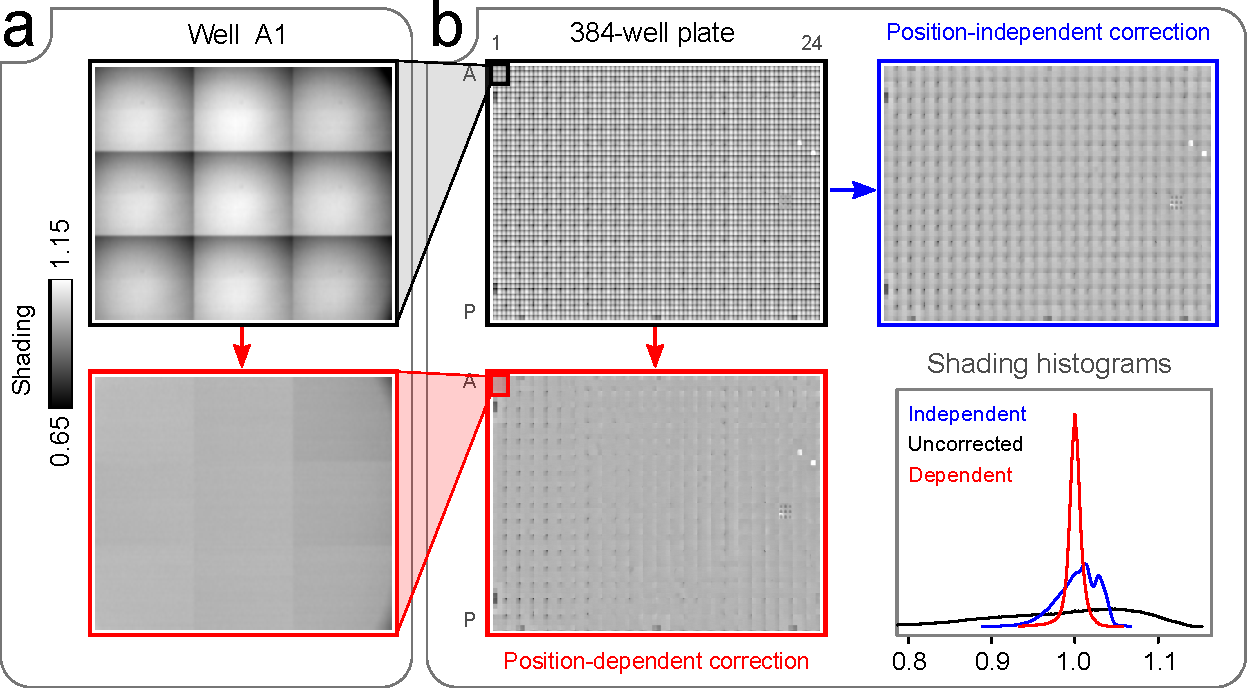
\includegraphics[width=6in]{FIGS/imaging/plateCorrection.pdf}
  {\singlespacing 
  \caption[ Demonstration of within-well positional image correction.]
            { For a within-well position, shading patterns are consistent
			throughout the entirety of a microtiter plate.
			I imaged 3x3 grids within every well of a 384-well
			plate containing dissolved fluorescein. Optical setup:
			black plastic 384-well plate (Corning \#3712), FITC filter,
			20X objective, Andor sCMOS camera.
			I cropped all images identically to remove pixels that contained
            well edges. Within-well images were montaged
			into a single image, and then normalized to the median pixel
			value of that montaged image (e.g. in \b{a}, top). This converts
			the images to an estimate of shading as defined in this chapter.
			Reference 3x3 image montages were
            made by taking the per-pixel average
			across all 3x3 montages (from all wells).
            This was done either with all 9 images in
			the 3x3 grid (Position-dependent correction) or with only the
			central image from the grid repeated 9 times
            (Position-independent correction).
			Finally, the resulting grids were montaged to show the image
			properties across the entire 384-well plate (\b{b}). Panel
			\b{a} shows larger thumbnails of the 3x3 image grids in well A1
			before and after position-dependent correction. The histograms
			in \b{b} shows the distributions of all relative pixel intensities
			in the montaged images. Tighter distributions indicate more
			accurate correction. White objects in the montaged images are
			auto-fluorescing debris; small black corners in remaining in
			corrected images are due to inclusion of a small portion
			of the black well edge.}
  \label{fig:imaging:plateCorrection}}
  \end{figure}


I was initially surprised at the high variability in shading patterns that I
observed within imaging datasets from microtiter plates.
In the literature there
appears to be an implicit assumption that such
variability is common and unpredictable,
as the most common correction methods used in big datasets are
per-image. However, shading is an artifact that is
generated by the light path, which is a static aspect of the microscope
optical setup, and so I would have expected it to be
unchanging within a dataset. Indeed, images taken at different positions along a
glass slide seem to show an unchanging shading pattern.
I therefore reasoned that it was the microtiter plates
themselves that modified the
shading pattern. Further, since microtiter plates are essentially
arrays of identical wells, I
predicted that the shading modification must be a function of the
image location
within a single well (as opposed to the position within the plate).
The source of the within-well shading modulation could be due to
reflections from well edges, local distortions
of the imaging surface, or lensing by
the solvent meniscus.


This prediction of within-well positional dependence of
shading patterns bore out, as can be seen in
\ar{fig:imaging:plateCorrection}. Further, this turned out
to be consistent for both 384- and 96-well plates from various
manufacturers and with different physical specifications
and materials. In 96-well plates
this positional effect is less dramatic, which is consistent with
shading patterns being modified by well edges (as these edges
are much further apart than are those in 384-well plates). I also note that
a position-independent correction method (that uses a single reference
image instead of one per within-well position,
\ar{fig:imaging:plateCorrection}, blue) dramatically improves
the images as well. Therefore this even simpler method may be suitable
for some datasets (though the resulting multi-modality in
\ar{fig:imaging:plateCorrection} could, in principle, generate
artificial cellular subpopulations \arp{introduction:variability}).




\subsubsection{Pipeline for within-well position-based image correction}
\label{correction:pipeline}

The within-well positional shading constancy allowed
me to implement a simple and robust image correction pipeline
for images from microtiter plates. This pipeline is based on the
existing reference-based approaches discussed above and in other
sources \cite{Bray2012,Bray2013}.




  \begin{figure}[!bt]
  \centering
  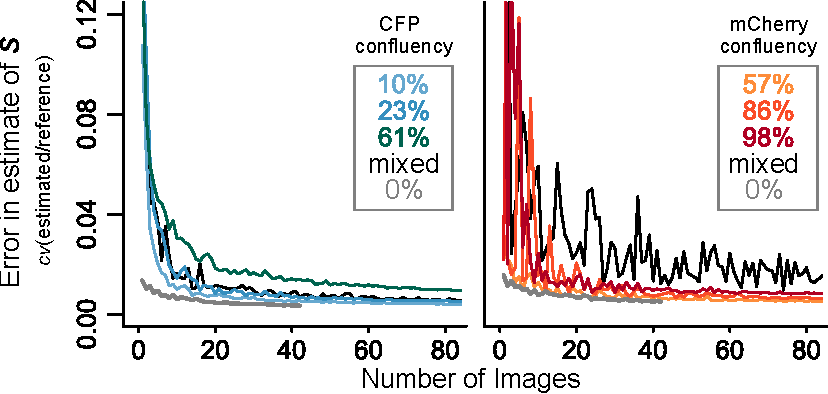
\includegraphics[width=5in]{FIGS/imaging/samplenum.pdf}
  {\singlespacing 
  \caption[ Estimating $S$ from sample-containing images.]
            { Shading ($S$) can be estimated using sample-containing
             images. Media-only wells are controls (0\% confluency).
             The spatially uniform fluorescence in these control wells was used
             to estimate the 
             ``reference'' shading by per-pixel averaging
             across 42 media-only control wells. I define
             ``confluency'' as the fraction of pixels in an image
             with intensities >3$\sigma$ above background.
             I used A549 cells expressing two differently-colored
             fluorescent proteins (left, nuclear CFP; right,
             cytosolic mCherry) at three different seeding
             densities (each seeding density had 84 replicates),
             effectively yielding six different confluency
             levels. I additionally created mixed-confluency
             image sets by randomly selecting across all
             confluency levels within each color channel.
             For each fixed number of images, $n$,
             selected from the same within-well position, I computed
             the ``estimated shading'' as the per-pixel median of
             $n$ randomly selected images. The error in the shading
             estimates are computed as the $cv$ of the per-pixel 
             ratio of (estimated shading)/(reference shading).
             For each confluency level, the inaccuracy of the
             sample-based shading estimate generally decrease
             with increasing numbers of images.}
  \label{fig:correction:samplenum}}
  \end{figure}

  

\begin{enumerate}

\item \textbf{Calibrate the microscope stage for the microtiter plate.}
Ideally, images should be acquired near well centers,
and relative within-well image positions should have
minimal drift between wells (e.g. images in well A1
should not be closer to the left well edge than those in H12).
It is important to be aware that this method will become
inaccurate with increasing positional drift. Also note that
microscope stage-driving software can vary in its accuracy,
and so custom solutions might be required for plates with
small wells.

\item \textbf{Measure the dark current component, $D$.}
The simplest approach is to capture images without a light
source, or with the light path diverted from the camera,
and per-pixel average the images. In practice, a small
number of images is sufficient ($n$=6-20 in my analyses).

\item \textbf{Subtract dark current, $D$, from all images in
the dataset.} The resulting images ($I-D$) are then modeled
by $S(B+F)$. This important step should be performed
regardless of the correction method subsequently
used, for the reasons explained above.
Without subtracting $D$, the estimated shading
patterns can become increasingly inaccurate with large
foreground values or small background values.

\item \textbf{Estimate shading $S$ for each distinct within-well
position.} This step is the most complicated in the pipeline
and should be performed with care. The goal is to obtain a
reference shading pattern for each within-well position.
For example, if an investigator has 9 images/well she will
need to estimate 9 shading patterns. There are at least two
possible approaches to this estimate.

\begin{itemize}

\item \textbf{Uniform reference images.} This approach
is the most robust, but is only possible if
there are extra wells that can be reserved solely for
acquiring reference images. In these extra wells, 
add dissolved fluorophore at the appropriate
concentration for the intended exposure time.
These wells should then be imaged along with the
other sample wells. In practice, I have found that a
small number (e.g. 6) of such uniform images is often
sufficient so long as the wells are free from fluorescing
debris. Across all wells $w$, for a given within-well
position $p$, the images $I_{w,p}$ should be per-pixel averaged
to obtain a reference image $\text{R}_p=\text{mean}_w (I_{w,p}-D)$.
Note that the per-pixel median or other quantile may
be more robust.

\item \textbf{Sample-based reference images.}
In high-throughput studies extra wells may be
unavailable for acquiring reference images.
In this case, the investigator can take advantage
of the large number of available sample images and otherwise
use the same method as for uniform reference images.
Because these sample images contain foreground, many
more values per coordinate are needed to get an
accurate estimate of shading. In \ar{fig:correction:samplenum}
I show how accuracy is dramatically affected by
the number of images used. The same figure suggests that
20-40 cell-containing images may often be sufficient, but this
is dependent on the cellular confluency of those images. 
\end{itemize}


The results of this step will be one reference image per
within-well position. As defined earlier, the shading values
should be centered on 1 to maintain the original intensity
range. Therefore once all reference images are collected
each image $\text{R}_p$ should be divided by the median
or mean of all reference image pixel values (with coordinates
$(r,c)$. The resulting shading patterns are described by
$S_p=\frac{\text{R}_p}{\text{mean}_{r,c,p} R_{r,c,p}}$


\item \textbf{Correct for the shading $S$ at each
within-well position.} To correct for shading,
every image $I_p$ should be per-pixel divided by
the corresponding shading pattern $S_p$ obtained in
the previous step: $\frac{I_p}{S_p}$. The resulting
images then contain only $B+F$.


\item \textbf{Subtract the background from each image.}
There are multiple approaches to this task.
The proper choice depends on the
particulars of the dataset, and so I illustrate two
cases here. In both cases, after subtracting background
we end up with the approximate foreground signal, $F$.

\begin{itemize}

\item \textbf{Global background subtraction.}
In some datasets, the background may vary little between
images. In this case, a global background value can be
estimated by averaging background pixels from a
representative image. Subtract this value from all pixels
in all images.

\item \textbf{Per-image background subtraction.}
In other datasets, there may be significant variability
in background from well to well. This could be due to errors
in staining or variation in exposure time. 
Background values can be estimated per image
by e.g. Otsu thresholding to automatically identify
background pixels \cite{Otsu1975}. Alternatively, a low
quantile pixel value can be taken as background
(the quantile choice is dependent on cell density).
Then, for each image, subtract its estimated
background value.


I note that, in the case of background
differences being due to something that would imply foreground
differences, such as due to exposure time or staining
variation, these per-image background estimates can be used
to normalize intensities between images. For example, to
normalize all images to some reference $B_{ref}$, determine the
normalization factor by taking its ratio with the per-image
background $B_{ref}/B_{sample}$. The image can then be multiplied by this
factor at every pixel, bringing it to the same intensity level
as the reference image. Care should be taken with this approach,
however, as it is not generally obvious when background variation
is predictive of foreground variation. 
\end{itemize}

\end{enumerate}

Note that this pipeline is only meant to remove shading $S$,
background $B$, and detector $D$ from images. What is left will
be all foreground layers, which may include various artifacts.
Further, the foreground values may vary for reasons independent
from imaging. For example, it is well established that assays
in microtiter plates can show batch, edge, row, and column effects.
These effects may non-biologically change the true values of $F$
and should thus be normalized after image correction
\cite{Malo2006,Dragiev2011,Dragiev2012,Carralot2012,Zhong2013}.

  
\subsection{Image correction quality control}

As with any data manipulation, the image correction
method outlined above should be checked to ensure
that no errors are introduced.
An obvious approach is to simply
visually inspect a subset of images, as in 
\ar{fig:imaging:flatfieldCheck}a,
though automated approaches are also feasible.


For background correction,
images should be checked to ensure that only the
background has been subtracted. This can be done
by examining background pixels. Since a perfect
subtraction will have set the centroid of the
background pixel distribution to zero, roughly half
of all post-correction background pixels should
be zero while the other background pixels take on small values.
Unfortunately, this task can be difficult to automate
for the same reason that errors may be introduced:
cell density may vary dramatically within a dataset,
complicating the automated identification of background pixels.


For shading correction, the likely artifacts will be
spatial. In other words, if there is over-correction
or under-correction,
this will cause certain regions of every image (and
the cells within those regions) to have systematically
higher or lower intensities than the global mean. This can be checked
in an automated way after cell segmentation by testing
for dependence of single-cell features on within-image
position (see an example of this approach in
\ar{fig:imaging:flatfieldCheck}b).



 \begin{figure}[!bt]
  \centering
  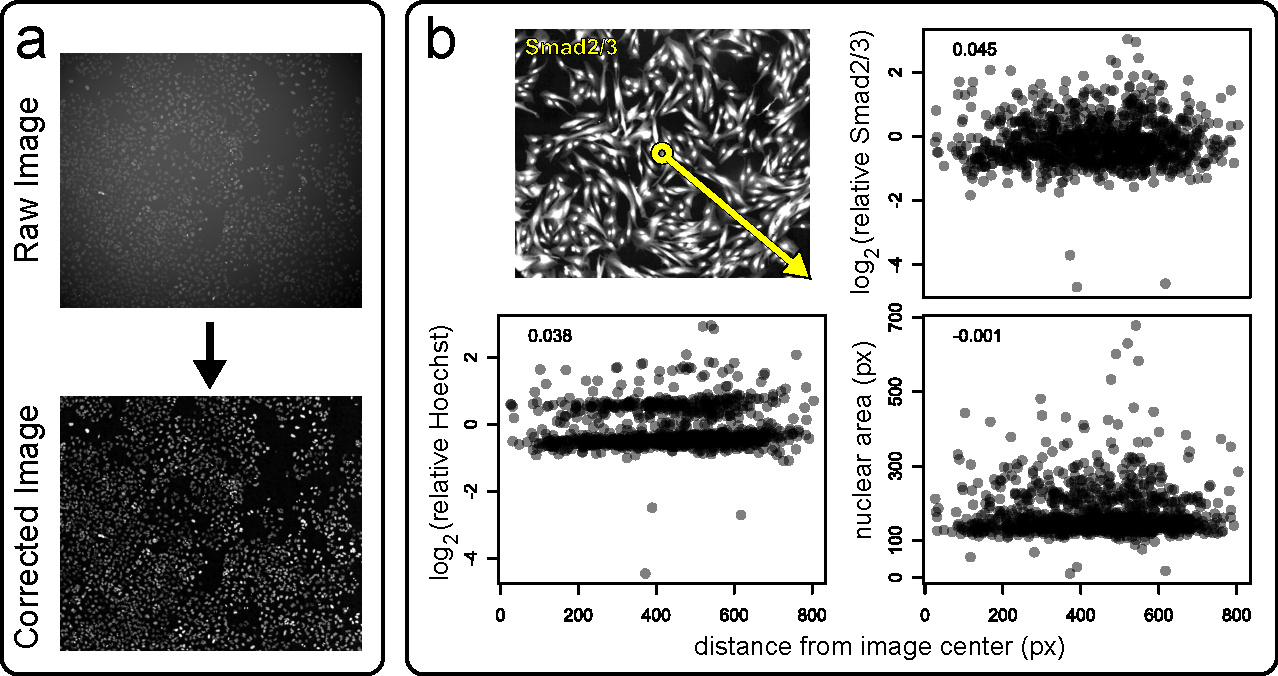
\includegraphics[width=6in]{FIGS/imaging/flatfieldCheck.pdf}
  {\singlespacing 
  \caption[ Quality control for image correction.]
            {Images can be over- or under-corrected, and
            therefore require quality control. \b{a},
            Visual inspection should reveal a flat background
            and a foreground that does not vary in a
            spatially predictable manner after correction. Histone H2B-Cyan
            Fluorescent Protein labeled A549 cells. Image
            courtesy Jungseog Kang (Altschuler \& Wu lab,
            UT Southwestern). \b{b},
            After segmentation and feature-extraction,
            single-cell features can be tested for within-image
            spatial dependence. Top left, a sample image of
            Smad2/3-stained human colonic epithelial cells,
            showing the radial metric of ``distance from image
            center.'' Plots show nuclear area and
            total nuclear Smad2/3 or Hoechst
            as a function of within-image radial position
            ($n$=1000/$\sim$20000 randomly-chosen cells).
            Intensities were median-normalized by well to prevent
            true experimental variation from affecting this
            test of positional phenotype dependence.
            Inset
            numeric value is the Pearson correlation coefficient
            for the two variables plotted. }
  \label{fig:imaging:flatfieldCheck}}
  \end{figure}